\chapter{Evaluating usefulness}\label{jiveEval}

This chapter will look at the external evaluation of \gls{jive} and the implemented changes, providing details on both the execution of the evaluation, and the results that were acquired.

\section{The test}\label{jiveEvalTest}
%mer konkret om hva som ble spurt om, spesifikke spørsmål
In order to evaluate both the usefulness of \gls{jive}, and the changes that were implemented, the evaluation was performed individually with a small group of six students.
The participants were initially recruited through a request sent to the participants of a second-year course that is mandatory for those who follow the informatics program.
This group was selected as they were matching the target group outlined in \cref{introduction}.
After only getting a single response, another request  was sent to the students association of the computer science program, bringing in the five remaining participants.
The latter group were all in their third year, and had already finished the \gls{hci}-course the previous semester.
This meant that they were familiar with the example programs, and had some knowledge of the MVC-pattern and how it behaves in Java-swing.
While this excluded the experiences of someone completely unfamiliar to these concepts, it did give the insight of relatively fresh experiences, as the participants remembered what they were finding hard to understand back then.

During the test, the students were given a demonstration of the main features of \gls{jive}, using implementations of the first, and the last exercise of the \gls{hci}-course as examples.
After getting familiar with \gls{jive}, they were shown the modified version, focusing on the new and modified features that were implemented.
They were then asked questions about how easily they understood the diagrams, and how useful they found the changes to be.
As well as whether the performance trade-off was acceptable for occasional use, if they could see themselves using \gls{jive}, and if so, in what situations.

The example programs both consisted of a simple user interface in swing, implementing the \gls{mvc} pattern.
Exercise 1 consists of a text field and two buttons to transform the text entered in that field to either uppercase or lowercase, and with an option to continually transform as new text is written.
Exercise 4 is an application that manages a simple list of people.
The interface it presents is split between a list of people, and a set of text fields to enter information about the selected person, as well as buttons to create new, and delete existing people.
Both of these programs, shown in \cref{fig:MMI-Oving-UI}, were relatively simple, with few events following directly from a user interaction, and as such, should have a limited performance reduction when used with \gls{jive}.
More complex programs are likely to suffer a greater performance impact from \gls{jive}, but are also out of the scope for the \gls{hci}-course.


\begin{figure}[H]
	\centering
	\begin{subfigure}{\textwidth}
		\centering
		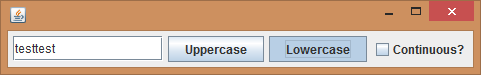
\includegraphics[width=\textwidth]{MMI-Oving1-UI}
		\caption{\gls{hci}-exercise 1}
		\label{fig:MMI-Oving1-UI}
	\end{subfigure}
	\begin{subfigure}{\textwidth}
		\centering
		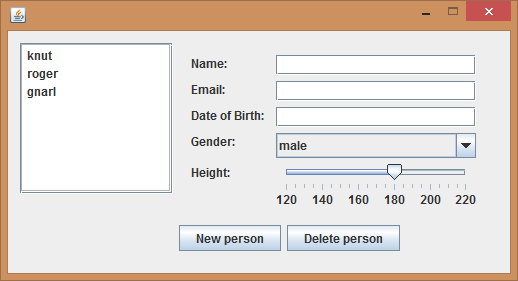
\includegraphics[width=\textwidth]{MMI-Oving4-UI}
		\caption{\gls{hci}-exercise 4}
		\label{fig:MMI-Oving4-UI}
	\end{subfigure}
	\caption{The two example programs used in the evaluation.}
	\label{fig:MMI-Oving-UI}
\end{figure}

\section{Results}\label{jiveEvalResults}

%nytte av diag
The evaluation resulted in mostly positive feedback, with every participant seeing some kind of use for a tool like \gls{jive}.
Of those in their third year, only one participant did not consider the use of diagrams to understand code to be useful.
In his experience, he learned just as well from reading the code directly, and building his own mental model of the program structure, but as he preferred simple text editors to \gls{ide}s, he could be considered to be outside of the target demographic.
On the other hand, he did recognize the usefulness of \gls{jive} as a tool to create documentation, and for presenting his own work to other participants in a project.
The rest of the participants shared the view that \gls{jive}, or a similar tool, could have been very useful when trying to understand the connection between \gls{gui} elements, listeners, and the actions that are triggered by them.
A few specifically mentioned that they found that connection to be difficult to understand.
One of them also had experiences as a student assistant, and recognized \gls{jive} as a tool that could give students a needed insight into what is going on in their programs.

The diagrams themselves were found to be both sufficiently detailed, and easy to understand, showing the available information in a simple and structured manner.
The tendency for the diagrams to grow large and unwieldy did become a problem, especially when running with the less restrictive filter, showing many of the swing-internals.
When hiding everything but user-created classes, the diagrams remained at an acceptable size, although the sequence diagram got quite long after a while.

%nytte av endringer
The implemented changes were generally well-received, with the ability to view a subsection of the sequence diagram in the isolated view being the most preferred change.
The changes to the filtering mechanism, while useful, were found to still be somewhat hard to use, due to the lack of an easy way of importing an existing filter, and the amount of work necessary to adapt a filter to the program being examined.
The modified labeling of object instances provided a small, but useful addition to the visible information.

%målt ytelse
\subsection{Performance}\label{jiveEvalPerf}
Regarding performance, it has already been shown in \cref{preMethods} that the tracing behavior of \gls{jive} must affect the analyzed program negatively.
The specific penalty varies with the complexity of the program, and the level of detail that is being logged.
The performance was measured as the it took for the program to reach a state where it could be interacted with.
Each of the example programs were run with both versions of \gls{jive}, and with two different levels of detail in the filter for the modified version, for a total of six measurements.
They were tested separately from the user evaluation, but on the same computer.
Each result was measured five times, with the averages reported in the table below:

\begin{table}[H]
	\begin{center}
		\label{tab:testPerf}
		\caption{Timing results from benchmarking}
		\begin{tabular}{llr}
			\hline
			Version of JIVE & Program & 5-run average\\ \hline
			Original JIVE & Exercise 1 & 5.0 s\\
			Modified JIVE, standard filter & Exercise 1 & 16.5 s\\
			Modified JIVE, swing-focused filter & Exercise 1 & 18.3 s\\
			Original JIVE & Exercise 4 & 8.2 s\\ 
			Modified JIVE, standard filter & Exercise 4 & 25.0 s\\ 
			Modified JIVE, swing-focused filter & Exercise 4 & 54.4 s\\ \hline
		\end{tabular}
	\end{center}
\end{table}

As these results show, there is a significant degradation in performance when going from the original version if \gls{jive} to the modified one.
The impact of letting a larger amount of events through the filter adds another solid penalty.
The reason for the latter has been explained in \cref{jiveFeatures}, and is simply a reflection of the added work of processing more events as they are let through the filter.
The impact observed from simply switching to the modified version can be explained by the way the filter mechanism was altered.
By first constructing a list of every package found in the workspace of the chosen program, and then use this list to add and remove excluded packages from the filter, the filter remains an exclusion filter, and its size reflects the size of the package list.
When \gls{jive} then checks to see if an event matches an entry in the filter, it has to look through a large amount of entries, and that clearly affects its performance.

%ytlese-meniger
As expected, the participants all agreed that the performance of \gls{jive} was too poor for continuous use, but they still found it acceptable for the occasional use that getting familiar with an example or documenting a project would require.
While a larger project could take several minutes to reach the initial stable state for a user to interact, one would only be interested in including the entire project when generating documentation for delivery.
By using the filter to ignore well known parts of the project, one could more easily show the interesting or complex parts while saving time.
In either case, the performance was not found to be a reason to never use \gls{jive}, but it would clearly depend on the complexity of the program, as well as what the filter would be letting through.

%problemer
\subsection{New issues}\label{jiveEvalIssues}
While the feedback from the participants was generally positive, they still found some areas that they thought could be further improved with new or modified functionality.

The mentioned challenge with importing an existing filter, was among the suggested changes.
Along with this, there was a desire to add a suggestion-functionality that would behave similarly to the autocomplete feature found in many search providers, including parts of Eclipse.
This feature would suggest package-names as the user started typing in the text field to add a new entry.

Another issue was the risk of diagrams becoming so large that they would be nearly impossible to navigate.
The size would especially become a problem when running larger programs, or when letting more objects through the filter.
To help with this, there was a desire to have the line of objects at the top of the sequence diagram visible at all times, regardless of how far down in the diagram one is currently looking, which would make the larger diagrams easier to navigate.
The ability to compress the height of the sequence diagram was also suggested.

Following the same lines, it was suggested that the placement of objects in the contour diagram could be reworked to give a more compact diagram.
\Cref{fig:MMI-Oving4-ObjectDiagVerybig} illustrates the problem, with a lot of unused space, and especially bottom row of objects extending far beyond the rest.
If the size of the diagram was restricted, for instance by preventing it from growing wider than the top row, preferring multiple shorter rows of objects instead of a few long ones.
This would let users see more information without scrolling the view of the diagram or zooming out.

\begin{figure}[h]
	\centering
	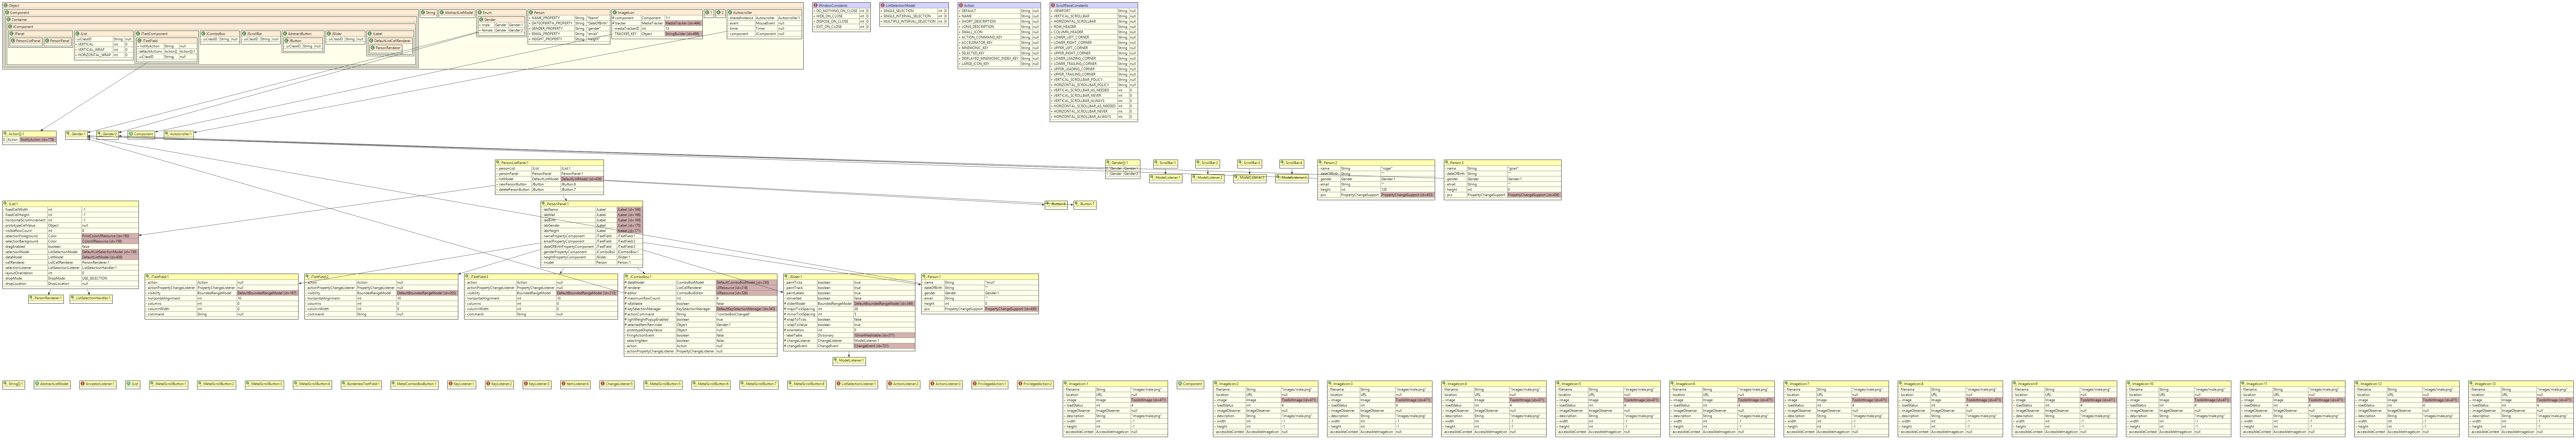
\includegraphics[width=\textwidth]{MMI-Oving4-ObjectDiagVerybig}
	\caption{Contour diagram that has grown unnecessarily large.}
	\label{fig:MMI-Oving4-ObjectDiagVerybig}
\end{figure}

Another suggestion was to make it possible to trigger the isolated view from the mentioned line of objects at the top of the sequence diagram instead of having to find the desired objects, and then scroll down to find the first event it is involved in.
